\section{Experiments and Evaluation} 
\label{sec:evaluation}
In this chapter we present and discuss the results of training the outlined neural network architecture for spoken language identification. We assess several performance metrics evaluated on our system.\\
Further, we experiment with modified model architectures to maximize the accuracy, improve its noise robustness and study the effect of background music on the neural network. To assess the real world performance of the the LID system we augment our data to simulate various noisy environments. Lastly, we show the classification performance of our approach and discuss the system's inter language discrimination and extensibility to other languages.     

\subsection{Hardware Resources}
\label{sec:hardware}
	In order to facilitate Keras' and TensorFlow's hardware-accelerated computation we executed all trainings on CUDA\footnote{\url{https://developer.nvidia.com/cuda-zone}, accessed 30.01.2017} compatible \ac{gpu} machines at our disposal at the Internet Technologies and Systems chair. Details can be found in table \ref{tab:hardware}.
		
	\begin{table}[h]
	\centering
	\begin{tabularx}{\textwidth}{lll}
	\toprule
	  		& Machine A 					& Machine B \\ \midrule
	OS  	& Ubuntu Linux 14.04 		& Ubuntu Linux 16.04 \\
	CPU  	& Intel\textsuperscript{\textregistered} Core\textsuperscript{\texttrademark} i7-4790K @ 4GHz 	& AMD FX\textsuperscript{\texttrademark}-8370  @ 4GHz \\
	RAM  	& 16GB 						& 32GB \\
	GPU  	& Nvidia GeForce\textsuperscript{\textregistered} GTX 980 	& Nvidia Titan X \\
	VRAM  	& 4GB 						& 12GB \\
	Images / sec &				& \\
	\bottomrule
	\end{tabularx}
	\caption{Hardware resources used in training the neural networks. We made heavy used of modern GPUs to benefit from quick hardware-accelerated numerical computations.}
	\label{tab:hardware}
	\end{table}
	\todo{measure images / sec}

\subsection{Data} 
\label{sec:data}
	For our performance evaluation we used the European Speech Repository and YouTube News dataset as described in chapter \ref{sec:datasets}. Both datasets were preprocessed and converted to spectrogram images as described in section \ref{sec:data_processing}. Each spectrogram image represents a non-overlapping ten second duration of source audio file. We chose this duration in reference to the NIST LRE2015 challenge\cite{lre2015}.	We split both datasets into a training (70\%), validation (20\%) and testing set (10\%) and all files were distributed equally between all four language classes. The number of samples per class was limited by the language with the least amount of files to ensure an equal class distribution. The European Speech repository yielded a total of ca. 19.000 training images  which amounts to roughly 53 hours of speech audio. The YouTube News dataset is considerably larger and yields a total of about 194.000 training files, or 540 hours. Table \ref{tab:data_splits} contains the detailed dataset splits.

	\begin{table}[]
	\centering
	\begin{tabularx}{\textwidth}{lrr}
	\toprule
	  				& European Speech Repository & YouTube News\\ \midrule
	Training Set    & 18.788						 & 193.432 \\
	Validation Set  & 5.372						 & 55.272 \\
	Test Set        & 2.684						 & 27.632 \\
	\midrule
	Total           & 26.844						 & 276.336 \\
	\bottomrule
	\end{tabularx}
	\caption{The amount of samples for our training (70\%), validation (20\%) and testing (10\%) set for the respective datasets.}
	\label{tab:data_splits}
	\end{table}

	Given the European Speech Repository's smaller size we only used it initially to confirm the validity of our approach. At the point at which we were satisfied with the results we did not include it in the extensive robustness tests that we used for the evaluation on the YouTube News dataset. Moving on to a bigger challenge, we augmented the original audio of the news dataset with three different background noises to evaluate how well our model would hold out in non ideal, real world situations outside of a news broadcasting studio. For the first experiment we added generic white noise to data. For the second experiment we added noise to simulate an old phone line or bad internet connection during voice chat. Lastly, we added background music to the data. All experiments are described in detail below.


\subsection{Training of the Neural Network Model} 
\label{sec:training}
	Neural networks have a multitude of hyperparameters that influence the training results drastically. In this section we will briefly explain our choice of hyperparameters alongside other important training settings:

	\begin{description}
	\item[Optimizer] We used Adaptive Moment Estimation (Adam)\cite{kingma2014adam} as our optimization method to quickly and efficiently reach convergence of our model. Adam utilizes momentum during gradient updates to support a quicker convergence. We set the optimizer's parameters $\beta_1$ to 0.9, $\beta_2$ to 0.999, and $\epsilon$ to 1e-08. For the majority of trainings we used Adam and only resorted to SGD during finetuning when we needed more control over the learning rate schedule and wanted smaller weight updates.
	\item[Weights Initializer] All layer weights are initialized within the range (0, 1) using a normalized Glorot uniform initializer\cite{glorot2010understanding}, also know as Xavier initializer. This heuristic is designed to compromise between the goal of initializing all layers to have the same activation variance and the goal of initializing all layers to have the same gradient variance. This initialized the biases to be 0 and the weights $W$ at each layer with the following heuristic\cite[chapter 8.4, p. 303]{Goodfellow-et-al-2016}: $W \sim U (-\frac{6}{\sqrt{n_j + n_{j+1}}}, \frac{6}{\sqrt{n_j + n_{j+1}}})$, where $U[-a, a]$ is the uniform distribution in the interval $(-a, a)$ and $n$ is the size of the previous layer.
	
	\item[Data Normalization] The grayscale images are loaded using SciPy and normalized to value in the range of [0, 1]. The shape for all inputs needs to be uniform across all samples and is set to [500, 129, 1], unless otherwise noted. Data loading is handled through Python generators\footnote{\url{https://docs.python.org/3/glossary.html#term-generator}, accessed 30.01.2017} to keep the system's memory footprint low.
	\item[Learning Rate] We set the initial learning rate to 0.001. Given the Adam optimizer's dynamic learning rate adaption we expect the learning rate to be automatically increased or decreased after every iteration. Therefore, we did not specify a manual learning rate decay schedule.
	\item[Batch Size] We specified the batch size depending on the available VRAM of the training machine. We used a value of 64 images per batch for Machine A and 128 images per batch for Machine B. (See section \ref{sec:hardware} for the hardware specifications.) 
	\item[Weight Regularization] Weight Regularization comprises any modification we make to a learning algorithm that is intended to reduce its generalization error but not its training error. We employed the L\textsuperscript{2} norm\cite[chapter 7.1.1, p. 231]{Goodfellow-et-al-2016}, sometimes also known as weight decay, as a weight regularizer for all convolutional and fully connected layers to improve the models generality. This regularization strategy drives the weights closer to the origin by adding a regularization term to our loss function. We penalize our loss with a weight decay value of 0.001. Additional regularization happens through the use of batch normalization layers.
	\item[Epochs] We limited the model training to a maximum of 50 epochs when using the Adam solver. We usually reached convergence well below this threshold. For training sessions with SGD we increased this parameter considerably since the weight updates per epoch are smaller and more training iterations are needed to reach convergence. To speed up our workflow we employed an early stopping policy and stopped a training if the validation accuracy and loss did not increase/decrease within a ten epoch window.
	\item[Metrics] We observed the loss, accuracy, recall, precision, f1 measure for both the training and validation set during model training. All values were saved to log files and visualized as graphs in TensorBoard. A complete summary of all assessed metric can be found in section \ref{sec:metrics}.
	\item[Loss] As is common for multivariate classification all models were trained with a softmax cross-entropy loss function. \todo{explain more. in theoretical background. add ref to section}
	\end{description}


\subsection{Evaluation} 

\subsubsection{Evaluation Metrics} 
\label{sec:metrics}
In this section we discuss the evaluation metrics used throughout our experiments. All metrics are generally only defined for binary classification scenarios. Given our multi-class classification problem we will report the average of the individual class performance measures in the following sections. 

\begin{description}
    \item[Accuracy] is a common measure in machine learning and is defined as the ratio of correctly classified samples to all samples in the dataset. In the context of language identification this translates as:
     

	$$
	\operatorname{accuracy} = \frac{
	   \vert \{ \text{correctly identified language samples} \} \vert
	  }{
	   \vert \{ \text{all language samples} \} \vert
	  }
	$$
     
    
    \item[Precision and Recall] Precision defines the ratio of retrieved language samples that are correctly identified as belonging to said language. Recall is the fraction of correctly identified language samples to all samples belonging to this language. Both measures are calculated using true and false positives as well as false negatives. These are defined as follows. \textit{True positives} are all samples belonging to one language which were correctly identified as belonging to said language. In contrast, \textit{false positives} are samples belonging to a language which were identified as belonging to another language. Lastly, \textit{false negatives} are the samples belonging to a language which were incorrectly identified as not belonging to said language.

	    $$
	    \operatorname{precision} = \frac
	      {\operatorname{true} \operatorname{positives}}
	      {\operatorname{true} \operatorname{positives} + \operatorname{false} \operatorname{positives}}
	    $$
		
		$$
		\operatorname{recall} = \frac
			{\operatorname{true} \operatorname{positives}}
			{\operatorname{true} \operatorname{positives} + \operatorname{false} \operatorname{negatives}}
		$$    


    \item[The F1 Score] is the scaled harmonic mean of precision and recall. It is used to a have combined judgement of recall and precision, since it is generally not interesting to assess one without the other.
    
    	$$
    	\operatorname{F1} = 2 * \frac{\operatorname{precision} * \operatorname{recall}}{\operatorname{precision} + \operatorname{recall}}
    	$$

\end{description}

\subsubsection{Results for EU Speech Repository Dataset}
\label{sec:results_eu}
In order to verify our theoretic model of using convolutional neural networks for classifying audio data in the image domain we established a baseline with the smaller EU Speech Repository dataset. Previous work with CNNs showed that the careful arrangement of the neural network layers has a great effect on the final classification performance. If one does not use enough or sufficiently large layers the model is not able to properly distinguish between classes. Going too deep or using too large layer outputs increases the overall number of model parameters to a degree where both training time and classification performance suffers again. The goal of this experiment is to find favorable settings for the number of convolutional layers needed, the kernel size of the convolutions, the number of output maps of the convolutional layers and finally the number of features of the fully connected layer.

	\begin{figure}[]
  		\centering
    	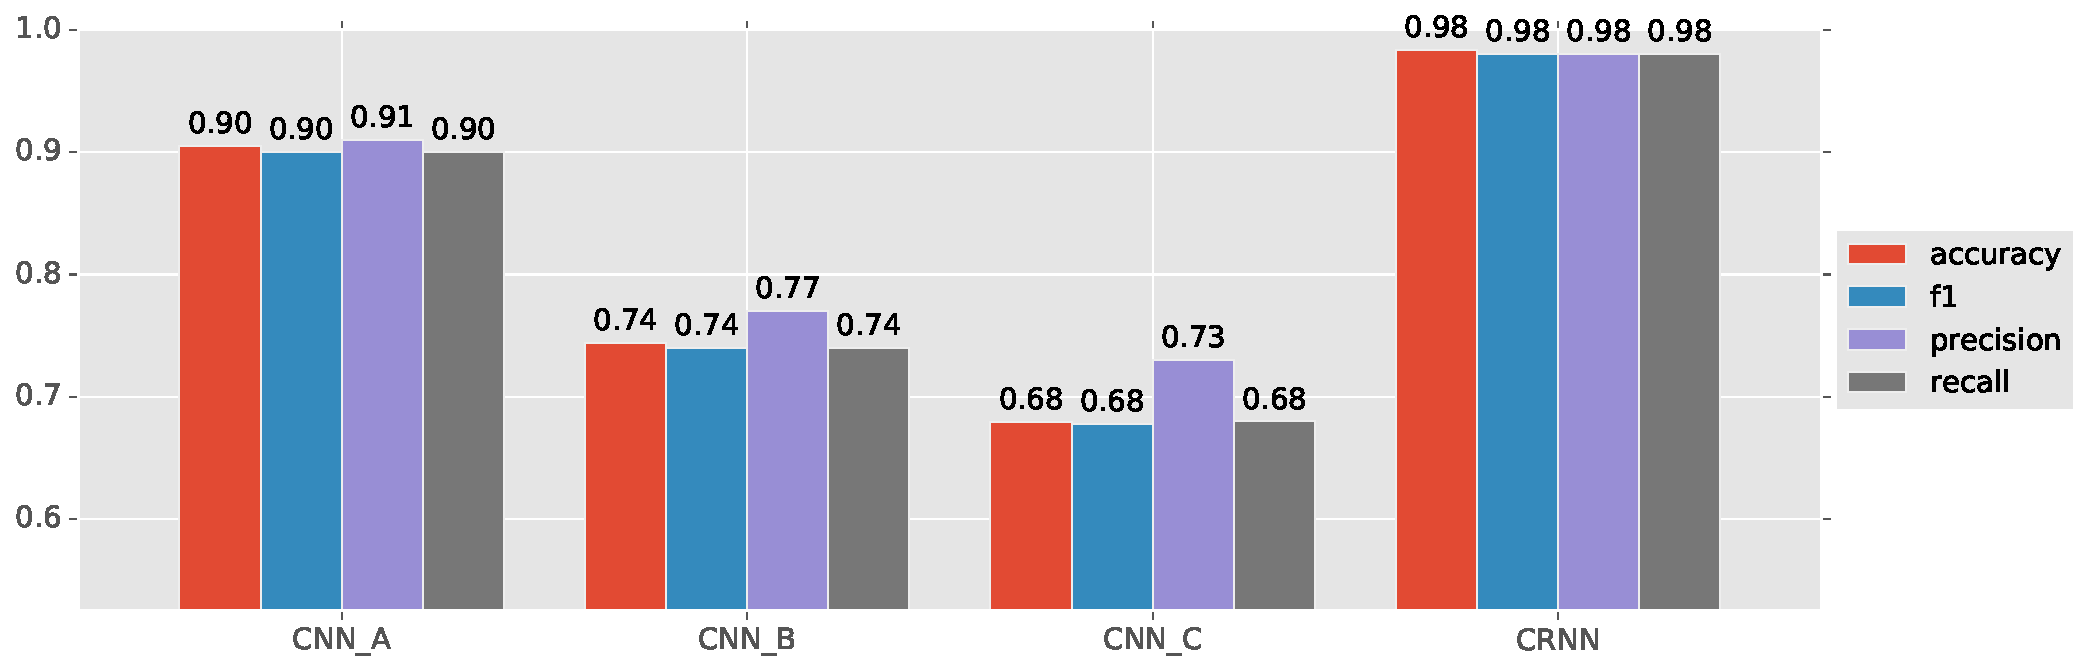
\includegraphics[width=\textwidth, keepaspectratio]{plots/results_eu_plot.pdf}
    	\caption{Performance measure comparison of three different CNN architectures evaluated on the EU Speech Repository dataset and our proposal of a \ac{crnn} model. CNN\_A outperforms all other CNN approaches with a top accuracy of 0.90, but is bested by the CRNN's 0.98 accuracy, showing the potential of this thesis' approach.}
    	\label{fig:eu_results}
	\end{figure}
	
	In section \ref{sec:cnn_architecture} we introduced three proposals for different CNN architectures. CNN\_A features large kernel sizes for the first two layers and we expect it to capture more information up front. A slightly smaller version of this design with less overall parameters is called CNN\_B. It served as an assertion to verify that CNN\_A's number of output feature maps were properly sized and not too large. Lastly, CNN\_C features equally sized kernels and boasts both more convolutional layers as well as an increased number of feature map outputs.

CNN\_A outperforms both of the other two network architectures with respect to all the evaluated performance measures, cf. figure \ref{fig:eu_results}. With a top-1 accuracy of 0.904 it trumps CNN\_B and CNN\_C with 0.743 and 0.68, respectively. Comparing the F1 score we get a similar result: 0.90 versus 0.74 and 0.68. This experiment confirmed a few of our initial hypotheses. Firstly, it proves that convolutional neural networks can be successfully used to classify audio data. Secondly, it demonstrates that spectrogram images are meaningful representations for audio that retain enough information for language identification. Thirdly, it shows that larger kernels for the initial convolutional layers are indeed favorable since the increased receptive field captures both the time and frequency domain better. 

Based on these findings we did some further testing with CNN\_A. Mishkin et al.\cite{mishkin2016systematic} were able to gain a small improvements in accuracy by exchanging convolutional layer's activation function. Therefore, we replaced our  Rectified Linear Unit (ReLU) activations to Exponential Linear Units\cite{clevert2015fast} (ELU) but were unable to measure any improvement (0.85 accuracy). 
Baoguan et al. \cite{shi2016end} proposed to use 1x2 rectangular pooling windows instead of the conventional square ones. This tweak yields feature maps with larger width, hence longer features along the time domain. In theory this should increase the CNN's sensitivity at capturing the occurrence of frequencies at certain time intervals. For this experiment we were unable to gain any improvement (0.81 accuracy), but we will come back to this technique for our CRNN approach later.

The task of this thesis was to evaluate the use of Deep Convolutional Recurrent Networks for language identification. Therefore we extended our previously best performing CNN\_A with a bidirectional \ac{lstm} layer to capture time steps both going forward from the start and going backward from then end of an audio segment. We interpreted the \ac{cnn} output as intermediate high dimensional representation of the audio frequencies and used every vector entry along the x-axis as a single step / input for the LSTMs as explained in section \ref{sec:hybrid_networks}. Confident in the features captured by our convolutional layers, we froze them during the CRNN training to disable any further weight updates for these layers. Instead, we focussed on only training the LSTMs weights and learn the frequency sequence of the audio sample. Our bidirectional LSTM layer trained two individual LSTMs with 512 outputs each, one training the input sequence from the start and one from the end. Both outputs were concatenated to form a single output vector with a dimension of 1024 which is followed by single fully connected layer for classification.\\
Our CRNN architecture outperformed all CNN approaches significantly. With a top-1 accuracy of 0.98 and a F1 score of 0.98 it proves the viability of the CRNN approach and reaffirms the central hypothesis of this thesis.


\subsubsection{Effect of Audio Duration} 
\label{sec:duration}
In all previous experiments we split the audio recordings into ten second segments, which translated to an image dimension of 500x129 pixels for the spectrogram. We decided on 10 second audio snippets to replicate on the setup of the \ac{nist} LRE 2015 \footnote{\url{https://www.nist.gov/itl/iad/mig/2015-language-recognition-evaluation}, accessed 15.02.2017} challenge. To study the effect of the audio duration on classification performance we set up two versions of the EU Speech Repository dataset with non-overlapping five and twenty second snippets but left the number of frequency bins unchanged. Hence, we changed the input dimensions to 250x129 pixels and 1000x129 pixels, respectively, and could not just use our previously trained models but had to retrain new models.

To set a baseline we used the same CNN\_A architecture as explained in the previous section. When completely training the five second version from scratch we achieved an accuracy of 0.81 falling short of the results achieved with ten second snippets. Next, we applied some transfer learning and finetuned CNN\_A on the new five second dataset. Since the convolutional layers are not bound to a specific input size and given that the frequency features did not change in dimension we were able to reuse the complete  convolutional weights. For the finetuning we froze the convolutional layers, confident in their ability to detect frequency features, and only retrained the final two fully connected layers. With the bisection of the input data the amount of model parameters were greatly reduced, especially the fully connected layer weights. To account for this we finetuned one model with a fully connected layer of 512 outputs and a second one with the default 1024 outputs. Overall this yielded an accuracy of 0.88 and 0.89, respectively. We concluded that the effect of the smaller fully connected layer is only marginally better. 

After establishing a solid CNN foundation we applied the same CRNN approach as previously highlighted. Due to the shorter audio duration the final pooling layer only features 5 output units along the x-axis compared to the 13 output units of the ten second CRNN. When interpreted as a sequence of time steps and fed into the bidirectional LSTM the accuracy improved only marginally to 0.90. We suspect that the number of time steps was too little to take full advantage of the recurrent network layer.\\
In an effort to increase the number of output units of the final pooling layer and hence increase the sequence length we applied 1x2 rectangular pooling tweak again. We changed the final two pooling layers and increased the number of output units along the x-axis to 22. The y-axis remained unaffected. The resulting accuracy of 0.90 and the F1 score of 0.91 remained comparable to the previous model and did not bring the desired effect. 

For the twenty second version we trained the network from scratch using the CNN\_A architecture. This yielded an accuracy of 0.90, which is comparable to its ten second counterpart. This experiment uses double the amount of pixels along the x-axis as the ten second baseline. This expansion of data led to an increase in computation time. At the same time, we felt that our LID system is more flexible when requiring shorter input audio snippets rather then longer one. We concluded that these longer snippets did neither improve our accuracy nor did they make the LID system more attractive overall.

In summary we believe that both decreasing and increasing the duration of the audio snippets used for training has a negative effect on the classification performance. While it is possible to train and finetune CNNs that match their ten second counterparts we found that the CRNN approach does not boost the model effectiveness in a similar manner.
	
	\begin{table}[]
	\centering
	\begin{tabularx}{\textwidth}{lrr}
	\toprule
  Model Architecture                            & Accuracy  & F1   \\ \midrule
  CNN (5s) from scratch                              & 0.81      & 0.81 \\
  CNN (5s) finetuned with 1024 Fully Connected Units & 0.88      & 0.89 \\
  CNN (5s) finetuned with 512 Fully Connected Units  & 0.89      & 0.89 \\
  CNN (20s) from scratch                             & 0.90      & 0.90 \\
  CRNN (5s) with 5 time steps                        & 0.90      & 0.91 \\
  CRNN (5s) with 22 time steps                       & 0.90      & 0.91 \\ \midrule
  CRNN (10s) for reference                           & 0.98      & 0.98 \\ 
 	\bottomrule
	\end{tabularx}
	\caption{Various CNN and CRNN model configurations trained on five second audio samples. The best performing five second CRNN still falls short of its ten second counterpart with an accuracy of 0.90 and 0.98, respectively.}
	\label{tab:audio_duration}
	\end{table}


\subsubsection{Results for YouTube News Dataset}
\label{sec:results_news}
Following the promising results from the experiments with the EU Speech Repository we switched to the ten times larger YouTube News dataset for further training and evaluation.\\
For our first experiment we used the same CNN\_A architecture as before but initialized the model weights with the weights of best performing model of the EU Speech Repository evaluation. Our reasoning here was to reuse the convolutional layers that were already trained to identify frequency ranges. However, with an accuracy of only 0.79 it did not perform as strongly as anticipated. One reason for this could be that the EU dataset is a lot smaller and does not feature as many diverse situations as present in news broadcasts. In the case of broadcasts all audio is recorded in a similar environment without much background noise and exhibits high signal quality.

Next, we trained the same CNN completely from scratch with randomly initialized weights. We had several setbacks when using an Adam optimizer and reverted to using standard SGD to keep our loss in check. Specifically, we encountered the exploding gradient problem\cite[ch. 8.2.4, p. 288]{Goodfellow-et-al-2016} and had to use gradient clipping to solve the issue. With this tweak we were able to get the model to converge and gained an accuracy of 0.9090 besting our previous attempt.\\ 
Given the larger size of the new dataset we also tried to increase the number of parameters by doubling the feature maps of the convolutional layers. This, however, did not help. As a next step we applied the CRNN approach again. Based on this CNN we added our bidirectional LSTM layers in the same manner as for the previous CRNNs and were able to slightly improve our accuracy and F1 score to 0.9124, respectively. 

To evaluate how our model architecture fares against established deep learning models we trained a model using Google's \emph{Inception-v3}\cite{szegedy2016rethinking} layout. This network design features more layers and is considerable deeper than our proposed CRNN architecture and is the result of Google's latest research into neural networks for image recognition tasks. Instead of a monolithic network design of sequential layers it uses a combination of parallel inception units, a sequence of convolution layers as one building block. Evaluating the \emph{Inception-v3} model resulted in a top accuracy of 0.9488 improving our results significantly. Applying the established CRNN treatment to this model increased the performance by roughly 1\% to an accuracy of 0.9579. In order to boost the performance even further we also tried a CRNN variation where both the convolutional layer weights and the LSTM weights were trained. In contrast to our initial CRNN approach this method also updates the existing convolutional filter. We found, however, that this variation did not improve performance. Figure \ref{fig:news_results} shows an overview of the performance metrics of the mentioned experiments.\\
The increased performance, however, does not come without a cost. With a total of 3.153.924 parameters our CRNN uses roughly six times less parameters then the \emph{Inception-v3} CRNN with its 19 million. This increases training time, requires more training data and consumes more GPU memory. On disk the serialized model weights come in at 30MB versus 260MB, which could be a potential disadvantage for deployment on mobile phones.

	\begin{figure}[]
  		\centering
    	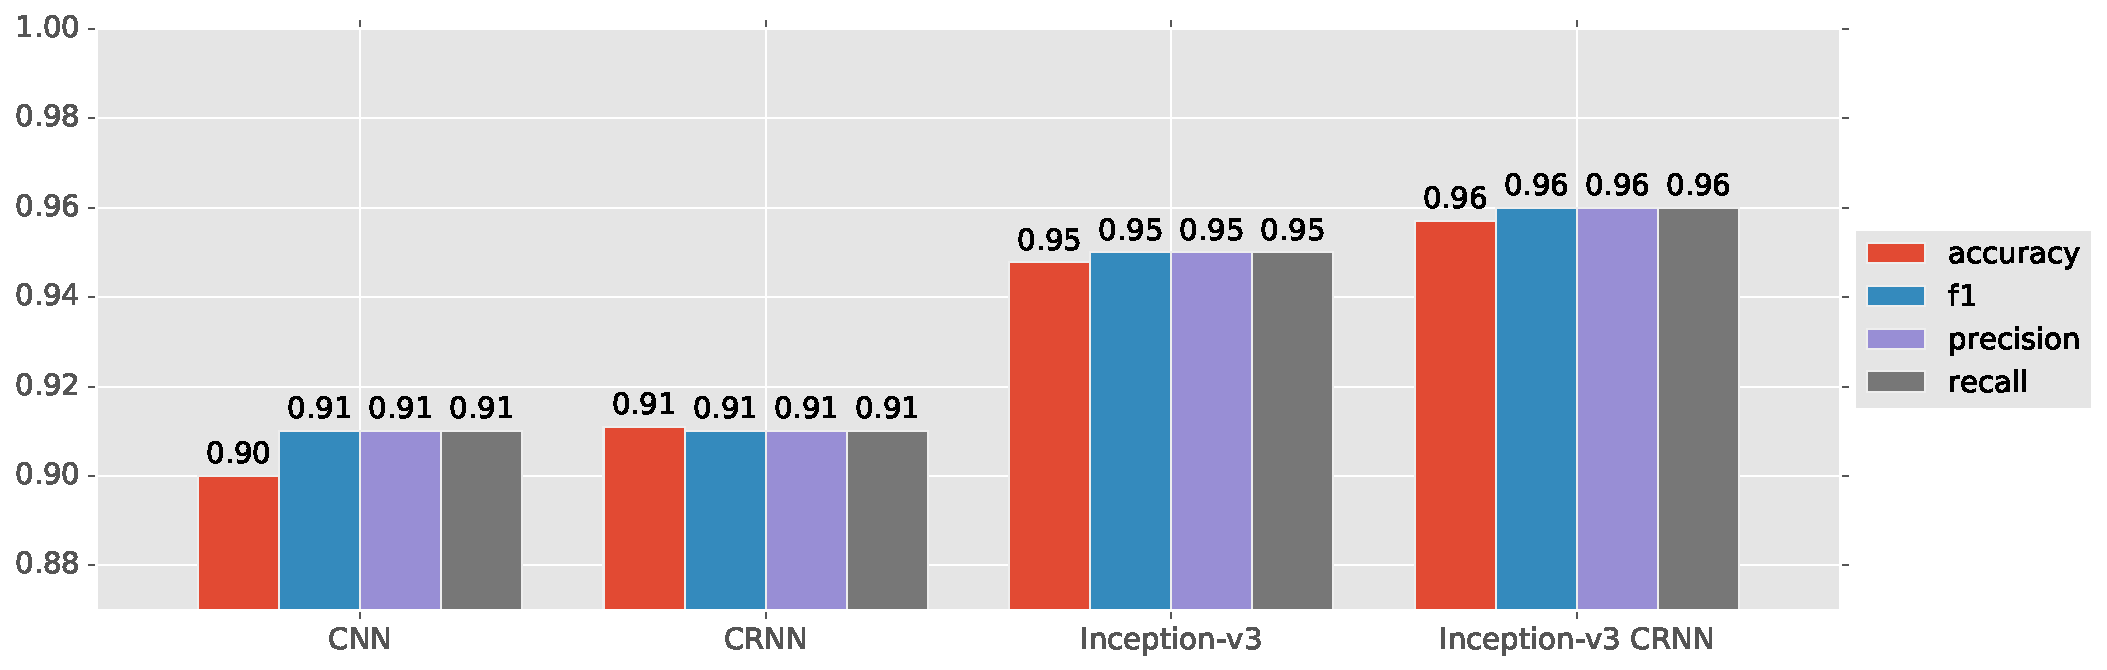
\includegraphics[width=\textwidth, keepaspectratio]{plots/results_news_plot.pdf}
    	\caption{Performance measurement comparison between our CNN and CRNN models and Inception-v3 based models. With a top accuracy of 0.96 the Inception style CRNN performs best but needs more than five times the amount of parameters compared to our proposed model architecture.}
    	\label{fig:news_results}
	\end{figure}


\subsubsection{Inter Language Discrimination} 
\label{sec:lang_discrimination}

Previous work\cite{montavon2009deep} raised concerns about the similarity of our four feature languages \textendash{} English, German, French and Spanish \textendash{} and the model's inability to discriminate between them properly. Both English and German belong to the West Germanic language family, while French and Spanish are part of the Romance languages. We hypothesized that our deep learning approach to language identification is able to differentiate between them reliably. \\
Table \ref{tab:language_family_crnn} shows the confusion matrix when evaluating language family pairs on the best performing CRNN. Spanish and French audio files separate very well with hardly any wrong classifications. Both languages are more likely to be classified as German and English rather then as the respective other, demonstrating that their learned representations are quite distinctive within their language family. \\
German and English language samples have a tendency to be misclassified as the respective other. Furthermore English also has a slight bias towards French, an observation in line with related work\cite{werkmeister2016practical}. German, however, distributes its classification error evenly between French and Spanish. Overall, German samples are misclassified the most across all languages.


	
	\begin{table}[]
	\centering
	\begin{tabularx}{\textwidth}{l|rrrr}
	      & EN     & DE     & FR     & ES \\ \midrule
    EN  & \cellcolor{lightgray} 6153   & 339    & 181    & 225 \\
    DE  & 426    & \cellcolor{lightgray} 6128   & 173    & 162 \\
    FR  & 200    & 145    &  \cellcolor{lightgray} 6447   & 107 \\
    ES  & 214    & 170    & 115    & \cellcolor{lightgray} 6399 \\
	\end{tabularx}
	\caption{Confusion matrix of our best performing CRNN. Ground truth values are along the row-axis. Predicted values are along the column-axis. English audio files are likely to be misclassified as German and vice versa. Both languages belong the family of Germanic languages. }
	\label{tab:language_family_crnn}
	\end{table}

	The confusion matrix for the Inception-v3 CRNN, table \ref{tab:language_family_inception}, match our observations for the other model. Again, German exhibits the most classification errors. 
	
	\begin{table}[]
	\centering
	\begin{tabularx}{\textwidth}{l|rrrr}
	      & EN     & DE     & FR     & ES \\ \midrule
	  EN  & \cellcolor{lightgray} 6648   & 140    & 45     & 61 \\
	  DE  & 152    & \cellcolor{lightgray} 6639   & 62     & 44 \\
	  FR  & 68     & 59     & \cellcolor{lightgray} 6742   & 27 \\
	  ES  & 75     & 83     & 42     & \cellcolor{lightgray} 6697 \\
	\end{tabularx}
	\caption{Confusion matrix of the Inception-v3 CRNN. Ground truth values are along the row-axis. Predicted values are along the column-axis. Despite its deeper architecture it makes similar classes of mistakes as our proposed CRNN. }
	\label{tab:language_family_inception}
	\end{table}
 

\subsubsection{Noise Robustness} 
\label{sec:noise_robustness}
Given that we left our raw audio data unchanged we expected a certain degree of noise within the dataset. Therefore we hypothesized that the neural network developed some noise robustness by itself. For instance, the convolution operations of the earlier layers summarize pixel values over an image patch and help with masking noise. To prove our theory we generated two augmented datasets based on the YouTube news dataset.\\ 
For the first one we mixed the audio signal with randomly generated white noise sound. The resulting audio samples are still easily identifiable for human listeners. The noise has a very strong audible presence, so much so that a human tester will easily be annoyed after a few seconds of listening to it.\\
For the second augmentation we added a more periodic cracking noise emulating analog telephony or a bad voice chat connection. We sampled a selection of fitting sound effects and randomly applied these to the source signal using the PyDub\footnote{\url{https://github.com/jiaaro/pydub}, accessed 01.03.2017} library. The resulting noise is not as noticeable and less intrusive as the white noise, but gives the augmented audio file a subdued vintage quality.

The white noise did deteriorate the language identification performance significantly both for our CRNN proposal and the Inception-v3 CRNN as can be seen in table \ref{tab:noise}. The noise spectrogram in figure \ref{fig:noise} show that the white noise effect has a very strong influence on the resulting image. Most parts of the image end up being covered by the distinct noise texture and only the lower frequency features remain intact. Yet most speech frequencies are still contained in this range. All pauses and fine grained details are also lost to the noise sound. The cracking experiment fared did not incur such a dramatic drop in performance. That might be in part due to the consistent recurring sound of the noise in contrast to the randomly generated white noise sound. Perhaps a second factor was the lower, less intrusive volume used for augmenting this dataset.

The deeper, more complex structure of the Inception-v3 CRNN did suffer a significantly smaller performance deterioration than our proposed CRNN model architecture. The more than five times as many parameters seem to capture the frequency features in a more robust manner. In an attempt to remedy the performance loss for our model we trained and finetuned models containing white noise data. We experimented with a 100\% noise dataset and the original news dataset extended with 10\% white noise for augmentation purposes. While both approaches did recover some white noise performance they reduced the general language identification and cracking noise statistics as a trade off.\\
Let it be noted that our audio mixing was fully automated and that the resulting samples varied in speech and noise volume. We tried to match volume levels of speech and noise to maintain as much clarity of speech as possible, yet some samples will have an artificial quality to them.

	\begin{figure}[]
  		\centering
    	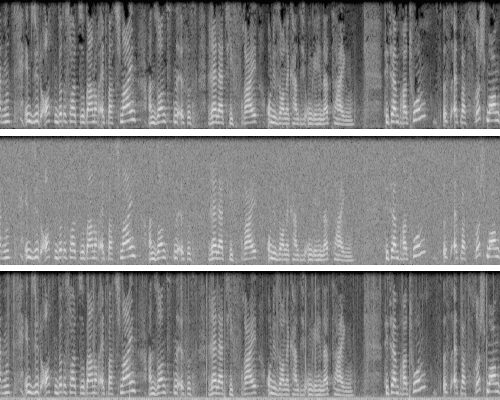
\includegraphics[width=\textwidth, keepaspectratio]{img/noise_spectrograms.png}
    	\caption{Spectrograms generated from the raw data, augmented with white noise and mixed with a cracking noise emulating analog telephony or a bad voice chat connection. The white noise aggressively subdues most higher frequencies and pauses causing a loss of classification performance. The cracking noise is less intrusive and therefore does not affect accuracy as much.}
    	\label{fig:noise}
	\end{figure}


Overall we note that even deep convolutional recurrent networks are still subject to the influence of noise on audio. We learned that our spectrogram preprocessing does not help in these situations and that different network architectures play an instrumental role in dealing with these situations.
 
	\begin{table}[]
	\centering
	\begin{tabularx}{\textwidth}{lrrrrr}
	\toprule
	Dataset & \multicolumn{2}{c}{CRNN} & \multicolumn{2}{c}{Inception-v3 CRNN} \\  
                & Accuracy  & F1    & Accuracy  & F1   \\ \midrule
No Noise		& 0.91		& 0.91	& 0.96		& 0.96 \\                
White Noise     & 0.63      & 0.63  & 0.91      & 0.91 \\
Cracking Noise  & 0.82      & 0.83  & 0.93      & 0.93 \\
 	\bottomrule
	\end{tabularx}
	\caption{Accuracy and F1 score for our models evaluated on the speech data augmented with two different types of noise. Our proposed model architecture is susceptible to noise and its performance deteriorates. The much deeper architecture of Inception-v3 CRNN is more robust against noise and retains a high performance.}
	\label{tab:noise}
	\end{table}



\subsubsection{Background Music Robustness}
\label{sec:music_robustness}

	\begin{figure}[]
  		\centering
    	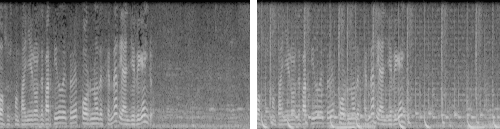
\includegraphics[width=\textwidth, keepaspectratio]{img/background_music.png}
    	\caption{Spectrograms generated from the raw data and augmented with background music noise. The added background music is clearly visible in the resulting spectrogram and changes the classification performance. Note that the previously silent part on the right-hand side now shows frequency activations as well. Additionally, the original ripple-like patterns become a lot more subdued and unclear. Further, new frequency activation patterns along the bottom of the image become visibile.}
    	\label{fig:background_music}
	\end{figure}
	
Many real world audio applications involve some form of music. For example, imagine speaking into your mobile phone from a busy cafe with background music or doing a voice chat session at home while the TV is running. Therefore we evaluated our model to see if language identification was still possible when mixing speech with music. For this experiment we used two different test sets. For the first series we augmented our existing YouTube news dataset with randomly sampled background music similarly to the background noise augmentation. The background audio was obtained from Soundcloud\footnote{\url{https://soundcloud.com/royalty-free-audio-loops}, accessed 01.03.2017} and features royalty free, instrument-only music from various genres, including Pop, Dubstep, Rock and Electro, amongst others.\\ 
We normalized the volume of these tracks and overlaid them onto our speech data while trying to stay below the speech audio volume. In the best cases the two audio streams blend nicely with the background music producing a soft but noticeable ambient effect, while retaining the clarity of the speech. In some other cases the audio levels and volume are over-accentuate for one or the other. The final result, however, does neither resemble a song nor a piece of music. We changed neither the tempo nor the pitch of our speakers and the rhythm of the vocals does not match the rhythm of the background audio. Given that our training set does not intentionally include samples with music or songs we expected the performance do be lower then for pure speech samples. Additionally it should be noted that the frequency activations of the instruments overlap with the speech frequencies. There is no easy way to separate the instruments from the singer or speaker in a music recording. The approach described here does not work for language identification on songs and we leave this task open for future work. Figure \ref{fig:background_music} shows the raw and augmented spectrograms of a Spanish speech snippet. There are several changes of note. First, the large area on the right hand side that was formerly silence starts to show repeated patterns. Second, along the lower image boundary we see new regular frequency activation spikes. Third, the clear ripple-like patterns in the raw spectrogram turn into muddy, unclear patterns.

	\begin{table}[]
	\centering
	\begin{tabularx}{\textwidth}{lrrrr}
	\toprule
Dataset & \multicolumn{2}{c}{CRNN} & \multicolumn{2}{c}{Inception-v3 CRNN} \\   
                  & Accuracy  & F1    & Accuracy   & F1   \\ \midrule
No Music		  & 0.91		  & 0.91	  & 0.96	  & 0.96 \\                     
Background Music  & 0.70      & 0.70  & 0.89  & 0.89 \\
 	\bottomrule
	\end{tabularx}
	\caption{Accuracy and F1 score for our models evaluated on the speech data augmented with background music from different genres.}
	\label{tab:audio_duration}
	\end{table}

\subsubsection{Model Extensibility} 
\label{sec:extensibility}
So far, all our experiments were conducted on datasets consisting of only four languages: English, German, French and Spanish. We extended the existing set with two new languages spoken by millions around the globe: Mandarin Chinese and Russian. The goal of this experiment was to learn whether we could expand our model to other languages. \\
We increased our existing YouTube news dataset with samples taken from Chinese and Russian news channels which now altogether forms the extended YouTube news dataset described in section \ref{sec:youtube_news}. In order to maintain the class distribution for six languages we had to decrease the number of training samples of the existing samples slightly. Table \ref{tab:dataset_comparison} contains the details for the extended YouTube news dataset.

For this experiment we first finetuned our previous best CNN by replacing the final fully connected layers and adjusted the number of output nodes to accommodate for six classes. The resulting model served as the basis for training the CRNN in a similar manner as in earlier experiments. Applied on the test set we measured an accuracy of 0.92 and F1-score of 0.92. Both measurements match our previous evaluation with four languages on the YouTube news dataset as laid out in section \ref{sec:results_news} proving that the proposed CRNN architecture can be extended to cover more languages. Figure \ref{fig:6lang} shows individual performance measures for each language. Mandarin Chinese outperforms all other languages with a top accuracy of 0.96, which could be interpreted as it sounding the most contrasting to western languages and featuring its own unique intonation. We also noted that Russian was most frequently misclassified as Spanish and vice-versa. In contrast to our previous observation German is no longer the worst performing class, but English takes that role now. This is in part due to a significant number of misclassification as Russian samples.

	\begin{figure}[]
  		\centering
    	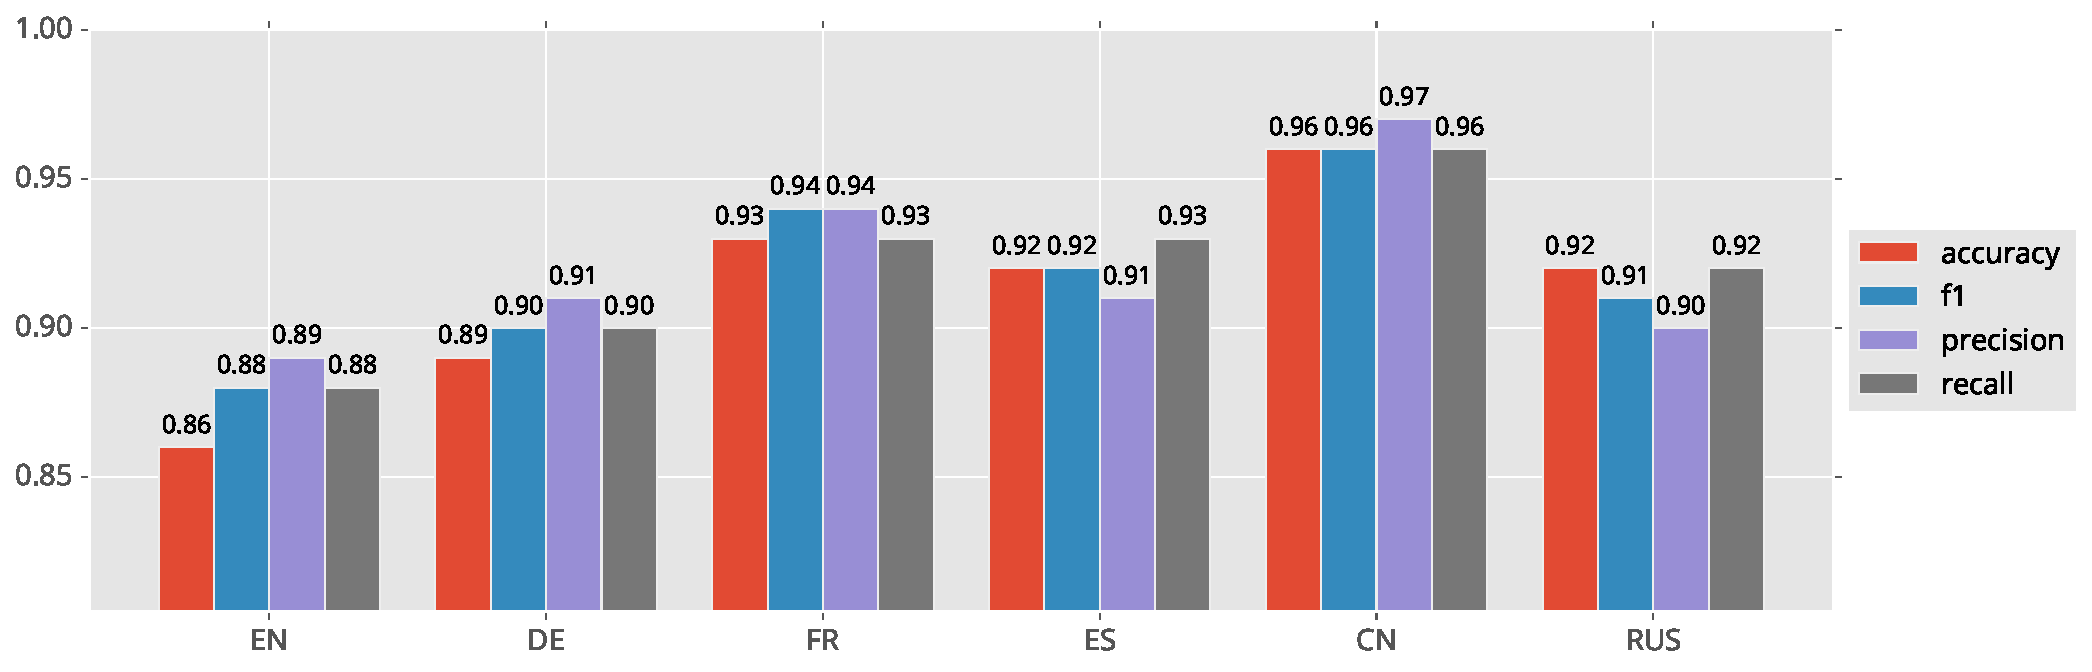
\includegraphics[width=\textwidth, keepaspectratio]{plots/results_6lang_plot.pdf}
    	\caption{Individual performance measurements for each of our six target languages: English, German, French, Spanish, Mandarin Chinese, and Russian. Chinese exhibits the best misclassification rate while English performs the worst. Overall the model performance is consistent with previous evaluations on four languages as highlighted in section \ref{sec:results_news}.}
    	\label{fig:6lang}
	\end{figure}

Given that both new languages are rooted within their own respective language families and feature considerable different intonations we were content to find that the features learned by our model are indeed universal in nature. We are confident in the believe that the approach to language identification proposed in this thesis can be successfully applied to a wide variety of languages.

\subsubsection{Visualizations} 
\label{sec:visualization}
All previous sections described and evaluated our model by measuring various performance indicators and applying them to different datasets. In this section we will present plots underlining earlier observations from a visual perspective.
	
	\begin{figure}
	\centering
	\begin{minipage}{.5\textwidth}
	  \centering
	  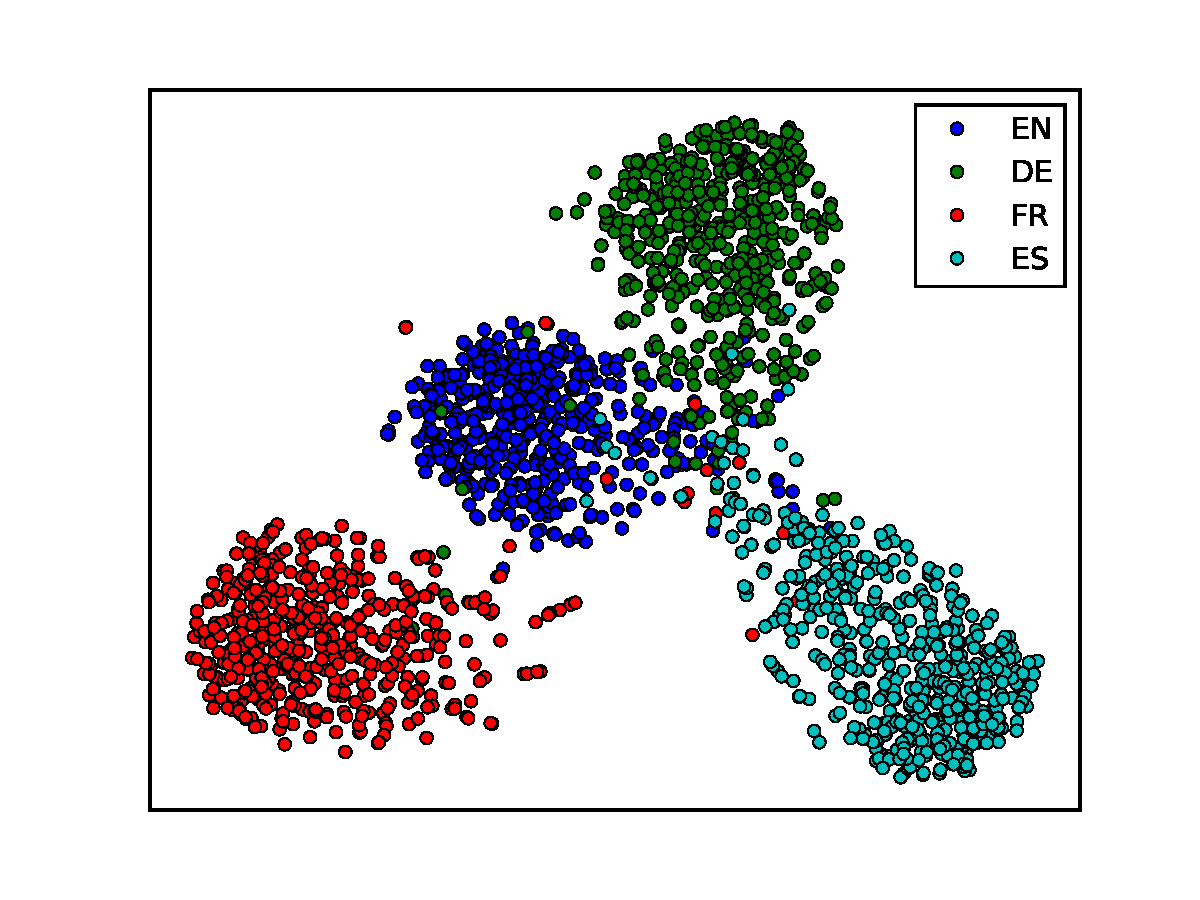
\includegraphics[width=\linewidth]{plots/tsne.pdf}
	\end{minipage}%
	\begin{minipage}{.5\textwidth}
	  \centering
	  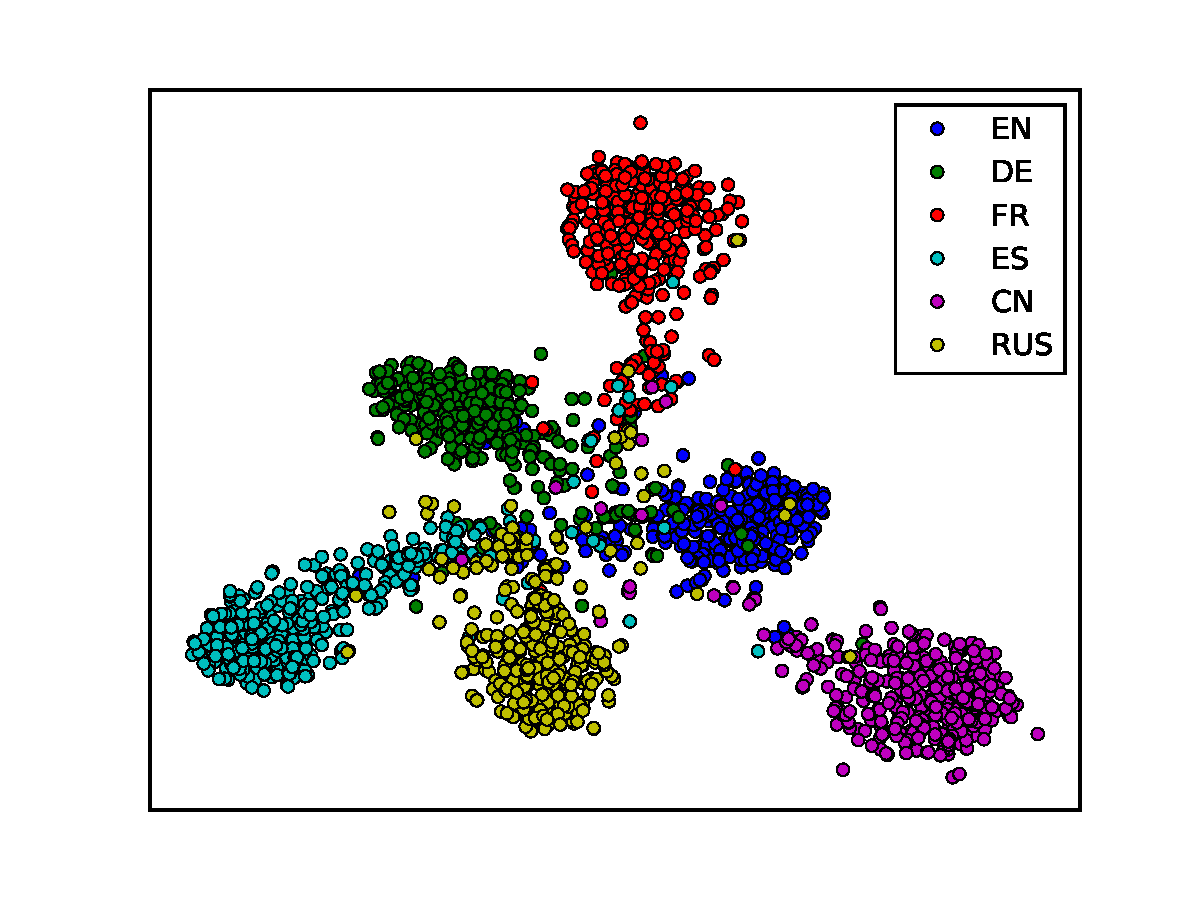
\includegraphics[width=\linewidth]{plots/tsne_6lang.pdf}
	\end{minipage}
	\caption{Two-dimensional t-SNE plots of the high dimensional vector representation of our YouTube news samples for a model trained with four and six languages,  respectively. All language classes form distinct clusters confirming that the network learned effective representations of the audio features.}
	\label{fig:tsne}
	\end{figure}

First we visualized the high-dimensional language vector embedding space using the t-distributed stochastic neighbor embedding (\ac{tsne}) algorithm\cite{maaten2008visualizing}. t-SNE is a nonlinear dimensionality reduction technique employed to map high dimensional data into 2D or 3D space for plotting. We applied this machine learning algorithm to the first 2000 predictions of our second to last fully connected layer right before the classifier and managed to project our 1024 dimensional YouTube news data into a 2D space. Figure \ref{fig:tsne} shows the resulting plot highlighting a good separation of our four language classes as independent clusters confirming that our network learned effective representations of the audio features. Note that French and Spanish split very nicely while German and English have some overlap. This is in line with our previous observations of classification errors as described in section \ref{sec:youtube_news}.

A primary advantage of deep neural networks is their ability to identify and learn useful features without requiring a data scientist to manually define these. Therefore one does not need any prior knowledge of the domain, a fact that makes these techniques so powerful and versatile. From an outsider's perspective they can appear as a bit of a black box and it remains unclear which features they ultimately deem relevant. In order to gain a better understanding of our model we visualized its convolutional layers. Figure \ref{fig:conv_filter} visualizes nine of the highest activating filters of the final convolutional layer. To obtain these filters we performed back propagation from the output of each filter back to an input image. This yielded the gradients of the output of the filter with respect to the input image pixels. We used that to perform gradient ascent, searching for the image pixels that maximize the output of the filter following the method proposed by Chollet\ref{chol16}.

Visualizations for the lower-level convolutional layers resulted in images of very simple geometric shapes like lines and circles which matched our expectations. With increasing network depth each convolutional layer's features combined and evolved into more complex shapes resembling our input domain. In figure \ref{fig:conv_filter} we can identify the familiar ripple like patterns that form frequency activations over time. This proves that the network learned these structures as we hypothesized earlier. We can also identify that some filters specialize in high frequency whereas others focus on low frequencies. Furthermore, it can be observed that the filters only react to a short and specific span of time within the spectrogram, all of which are less than one second in duration.

	\begin{figure}[h]
  		\centering
    	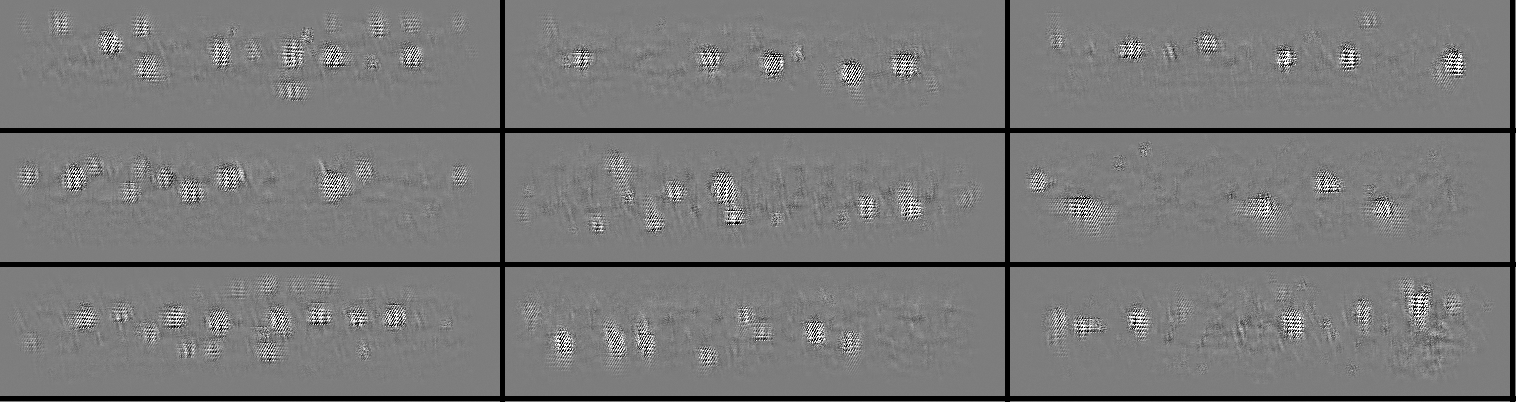
\includegraphics[width=\textwidth, keepaspectratio]{img/conv_filter.png}
    	\caption{Visualization of nine filters in the final convolutional layer. Note the ripple-like patterns responsible for detecting different frequency spans in the input audio.}
    	\label{fig:conv_filter}
	\end{figure}

\subsubsection{Discussion} 
\label{sec:comparison}
In this section we introduced and compared different CNN and CRNN architectures for language identification and proved that these models can be used to solve our research task to a satisfying quality. This thesis confirms that audio tasks can be solved within the image domain using spectrogram image representations. As hypothesized we were able to prove that our system learned the audio and frequency structures of these spectrogram images. We showed that these results hold true regardless of the input audio source and across various languages. Further, we  demonstrated that the learned intermediate language representations were indeed universal and not language specific and could easily be applied to other languages as well.\\
 Our approach of combining convolutional neural networks with bidirectional long short term memory cells showed a consistent improvement over baseline CNNs. In general we were able boost accuracy by at least 1\%. Furthermore, we established that an Inception-v3 style CRNN outperformed all other approaches both in terms of accuracy (0.96) as well as with noise robustness. 

We presented several augmented datasets to evaluate both noise and background music robustness. We were content to note that the noise resistance of the Inception-v3 CRNN reached acceptable levels without us having to modify or restructure our algorithm. This reaffirms our believe in deep learning techniques as a viable tool for audio tasks.

Our CRNN approach interpreted every vector entry along the x-axis as a separate time step for the recurrent layer. Hence, all results gathered here are representative of only ten seconds of an audio file. We believe that in a production ready system we could increase the prediction performance by doing a majority voting across multiple segments of a longer audio file.

